% Source: AESP_466_ClassWork/Supplements/Notes/latex/5.3.3/5.3.3.tex

\documentclass[border=4pt]{standalone}
\usepackage{amsmath,amssymb,amsthm}
\usepackage{graphicx}
\usepackage{tikz}
\usepackage{xcolor}
\usetikzlibrary{arrows.meta,calc,positioning,decorations.markings,patterns,shapes.geometric,angles,quotes}

\definecolor{Garnet}{HTML}{73000A}
\definecolor{USC_Rose}{HTML}{CC2E40}
\definecolor{USC_Blue}{HTML}{466A9F}
\definecolor{USC_Slate}{HTML}{1F414D}
\definecolor{USC_Olive}{HTML}{65780B}
\definecolor{USC_Lime}{HTML}{CED318}
\definecolor{USC_Gold}{HTML}{A49137}
\definecolor{USC_Black90}{HTML}{565556}
\definecolor{USC_Black10}{HTML}{ECECEC}

\newcommand{\vect}[1]{\mathbf{#1}}
\newcommand{\mat}[1]{\mathbf{#1}}
\newcommand{\uvec}[1]{\hat{\mathbf{#1}}}
\newcommand{\transpose}{^{\mkern-1.5mu\mathsf{T}}}
\newcommand{\inv}{^{-1}}
\newcommand{\deriv}[2]{\frac{d #1}{d #2}}
\newcommand{\pderiv}[2]{\frac{\partial #1}{\partial #2}}

\begin{document}
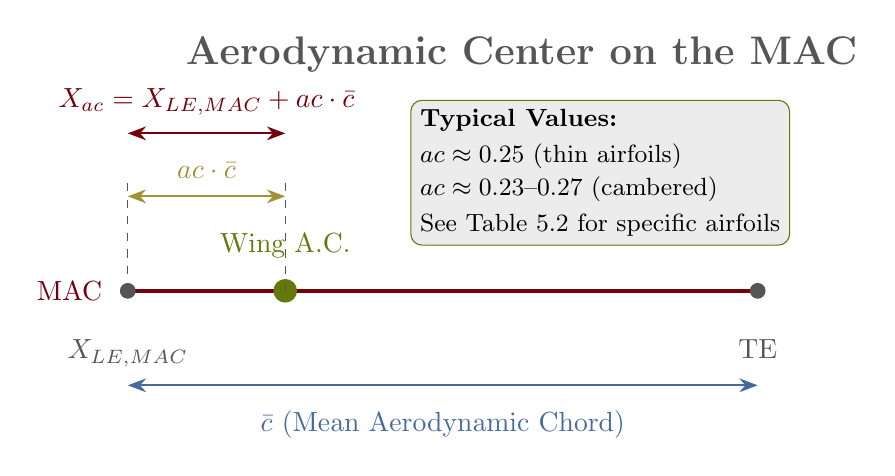
\begin{tikzpicture}[>=Stealth, scale=1.0]
    % Title
    \node[font=\Large\bfseries, USC_Black90] at (5,5) {Aerodynamic Center on the MAC};

    % MAC chord line
    \draw[ultra thick, Garnet] (0,2) -- (8,2);
    \node[Garnet, left] at (-0.2,2) {MAC};

    % Leading edge marker
    \fill[USC_Black90] (0,2) circle (0.1);
    \node[USC_Black90, below] at (0,1.5) {$X_{LE,MAC}$};

    % Trailing edge marker
    \fill[USC_Black90] (8,2) circle (0.1);
    \node[USC_Black90, below] at (8,1.5) {TE};

    % MAC length dimension
    \draw[<->, thick, USC_Blue] (0,0.8) -- (8,0.8);
    \node[USC_Blue, below] at (4,0.6) {$\bar{c}$ (Mean Aerodynamic Chord)};

    % Aerodynamic center location (at quarter chord)
    \fill[USC_Olive] (2,2) circle (0.15);
    \node[USC_Olive, above] at (2,2.3) {Wing A.C.};

    % ac * c_bar dimension
    \draw[<->, thick, USC_Gold] (0,3.2) -- (2,3.2);
    \node[USC_Gold, above] at (1,3.3) {$ac \cdot \bar{c}$};

    % Vertical reference lines
    \draw[thin, dashed, USC_Black90] (0,2) -- (0,3.4);
    \draw[thin, dashed, USC_Black90] (2,2) -- (2,3.4);

    % X_ac total dimension
    \draw[<->, thick, Garnet] (0,4) -- (2,4);
    \node[Garnet, above] at (1,4.1) {$X_{ac} = X_{LE,MAC} + ac \cdot \bar{c}$};

    % Typical value annotation
    \node[draw=USC_Olive, fill=USC_Black10, rounded corners, align=left, font=\small] at (6,3.5) {
        \textbf{Typical Values:}\\[0.2em]
        $ac \approx 0.25$ (thin airfoils)\\[0.1em]
        $ac \approx 0.23\text{--}0.27$ (cambered)\\[0.2em]
        See Table 5.2 for specific airfoils
    };

\end{tikzpicture}
\end{document}
